% ========== EDERFUGL ==========
\begin{frame}{%
  \begin{minipage}[c]{0.30\textwidth}
    Ederfugl
  \end{minipage}%
  \hfill
  \begin{minipage}[c]{0.45\textwidth}
    \footnotesize
    \textbf{Jagttid:} 1.\ oktober -- 31.\ januar \\[0.15em]
    {\scriptsize (kun hanner; hunner fredet)}
  \end{minipage}%
  \hfill
  \begin{minipage}[c]{0.15\textwidth}
    \noindent\raggedleft
    
\includegraphics[width=0.5cm, height=0.5cm, keepaspectratio]{Billeder/Ikoner/star.png}%
    \hspace{0.2em}%
    
\includegraphics[width=0.5cm, height=0.5cm, keepaspectratio]{Billeder/Ikoner/star.png}%
    \hspace{0.2em}%
    
\includegraphics[width=0.5cm, height=0.5cm, keepaspectratio]{Billeder/Ikoner/star.png}
  \end{minipage}%
}
  \vspace{0.25em}
  \begin{columns}[T]
    % --- Venstre kolonne: Tekst ---
    \column{0.55\textwidth}
    \setlength{\parskip}{0.5em}
    \tiny
    \RaggedRight
    \textbf{\textit{Somateria mollissima}} – største dykand i Danmark \par
    \textbf{Udseende:} \\
    \quad – Kok: Trekantet hoved, grønne aftegning i nakken, bølgeformede striber \par
    \quad – Høne: trekantet hoved, bølgeformede striber \par
    \textbf{Levesteder:} Kystfugl, på havet og i fjorde. \par
    \textbf{Føde:} Primært blåsmuslinger. \par
    \textbf{Udbredelse:} Både stationære og trækfugle. \par
    \textbf{Træk/standfugl:} Begge
    \begin{itemize}
      \itemsep0pt
      \item \textbf{Yngleforhold:} Yngler i hele Danmark.
      \item \textbf{Kønsmoden:} Ca. 3 år
      \item \textbf{Mono/polygam:} Monogam
      \item \textbf{Bestandsomsætning:} Langsom
      \item \textbf{Kuld:} 4–6 æg
      \item \textbf{Jagttid:} 1.\ oktober -- 31.\ januar (kun hanner; hunner fredet)
    \end{itemize}
    % --- Højre kolonne: To billeder ---
    \column{0.40\textwidth}
    \centering
    \fbox{%
      \begin{minipage}{\linewidth}
        \centering
        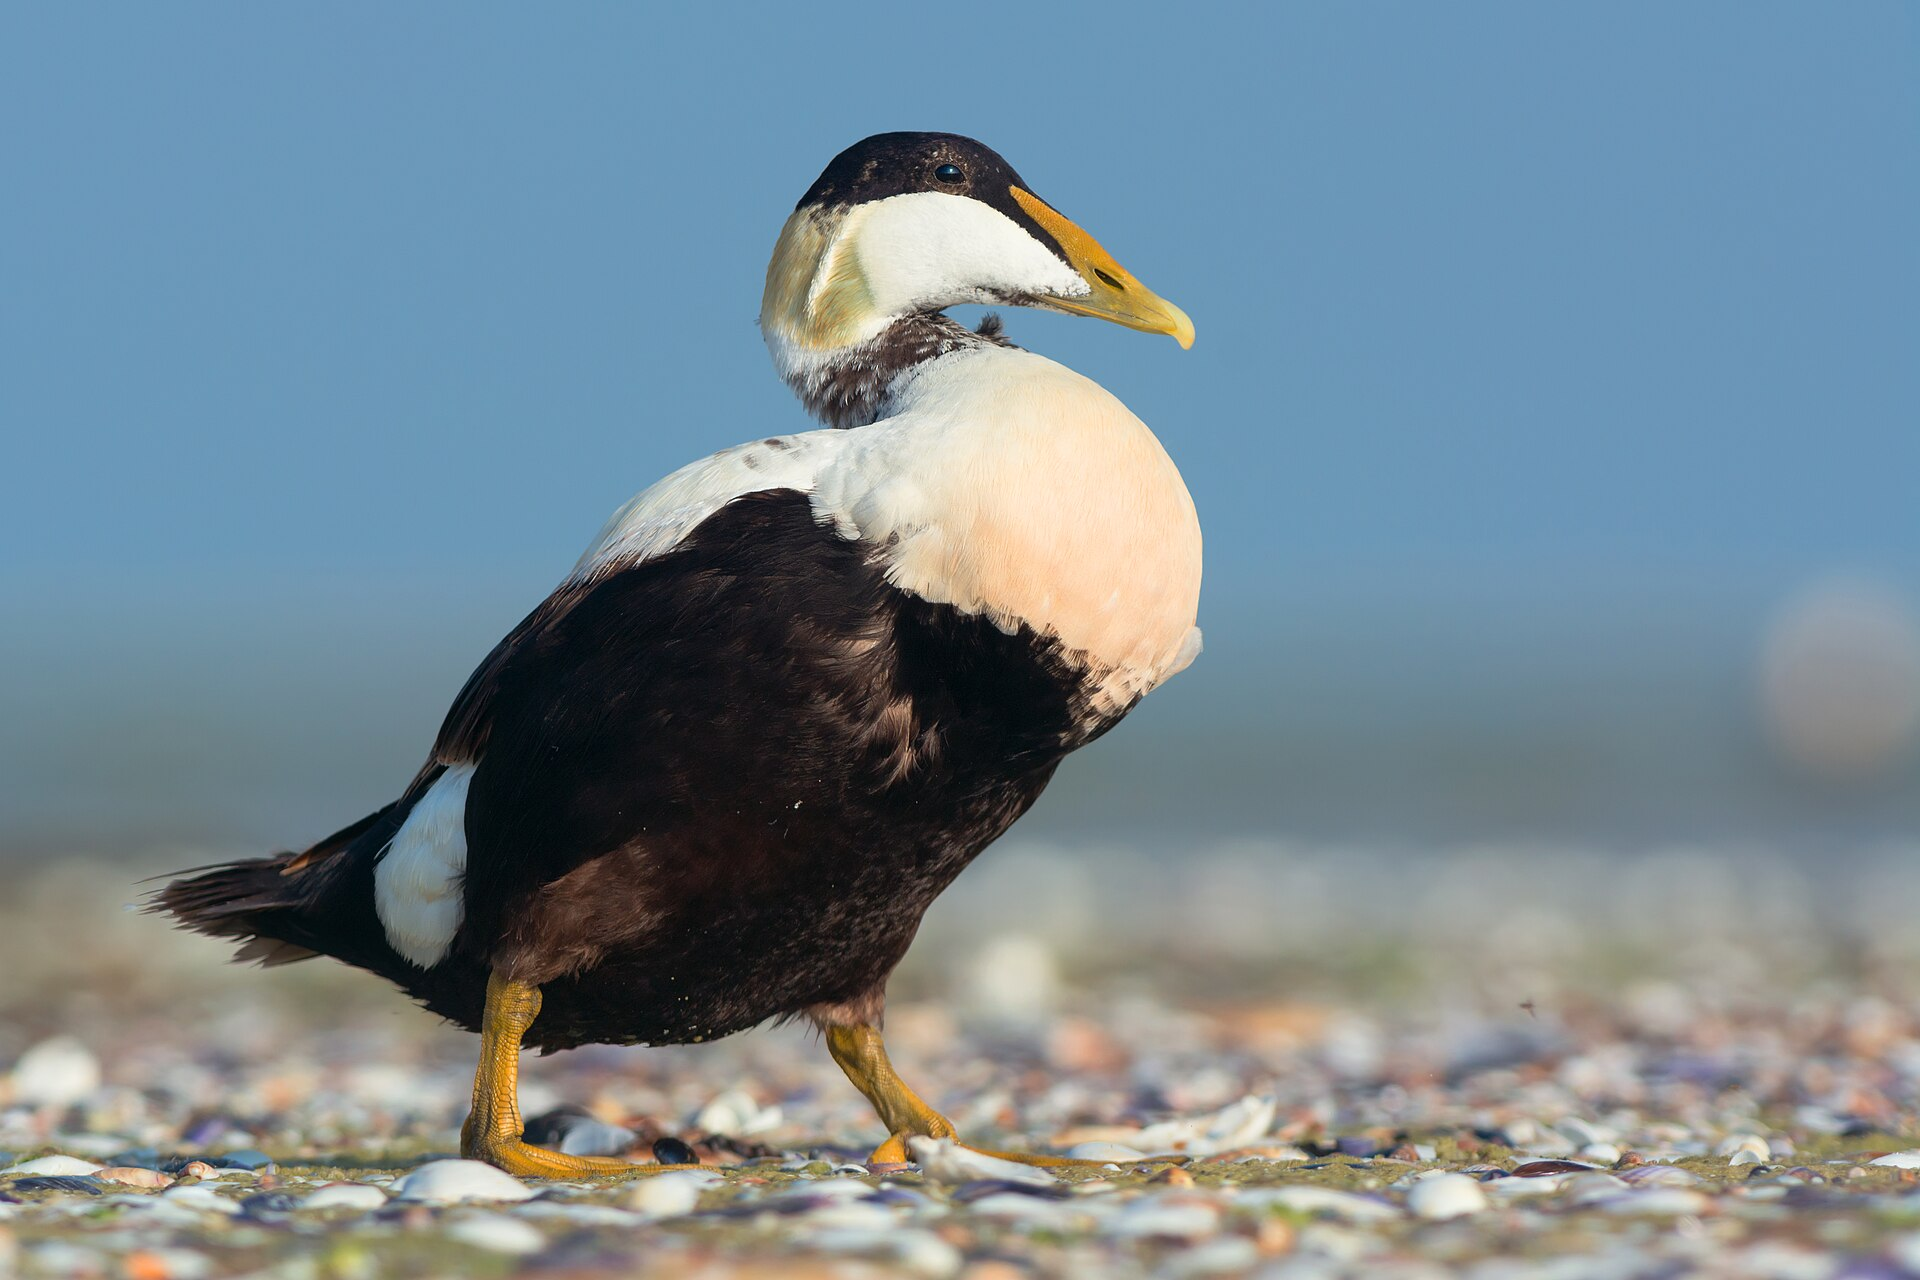
\includegraphics[width=0.7\linewidth, height=3cm, keepaspectratio]{Billeder/Dyr/Fugle/Aender/Dykaender/ederfugl_han.jpg}\\[0.5em]
        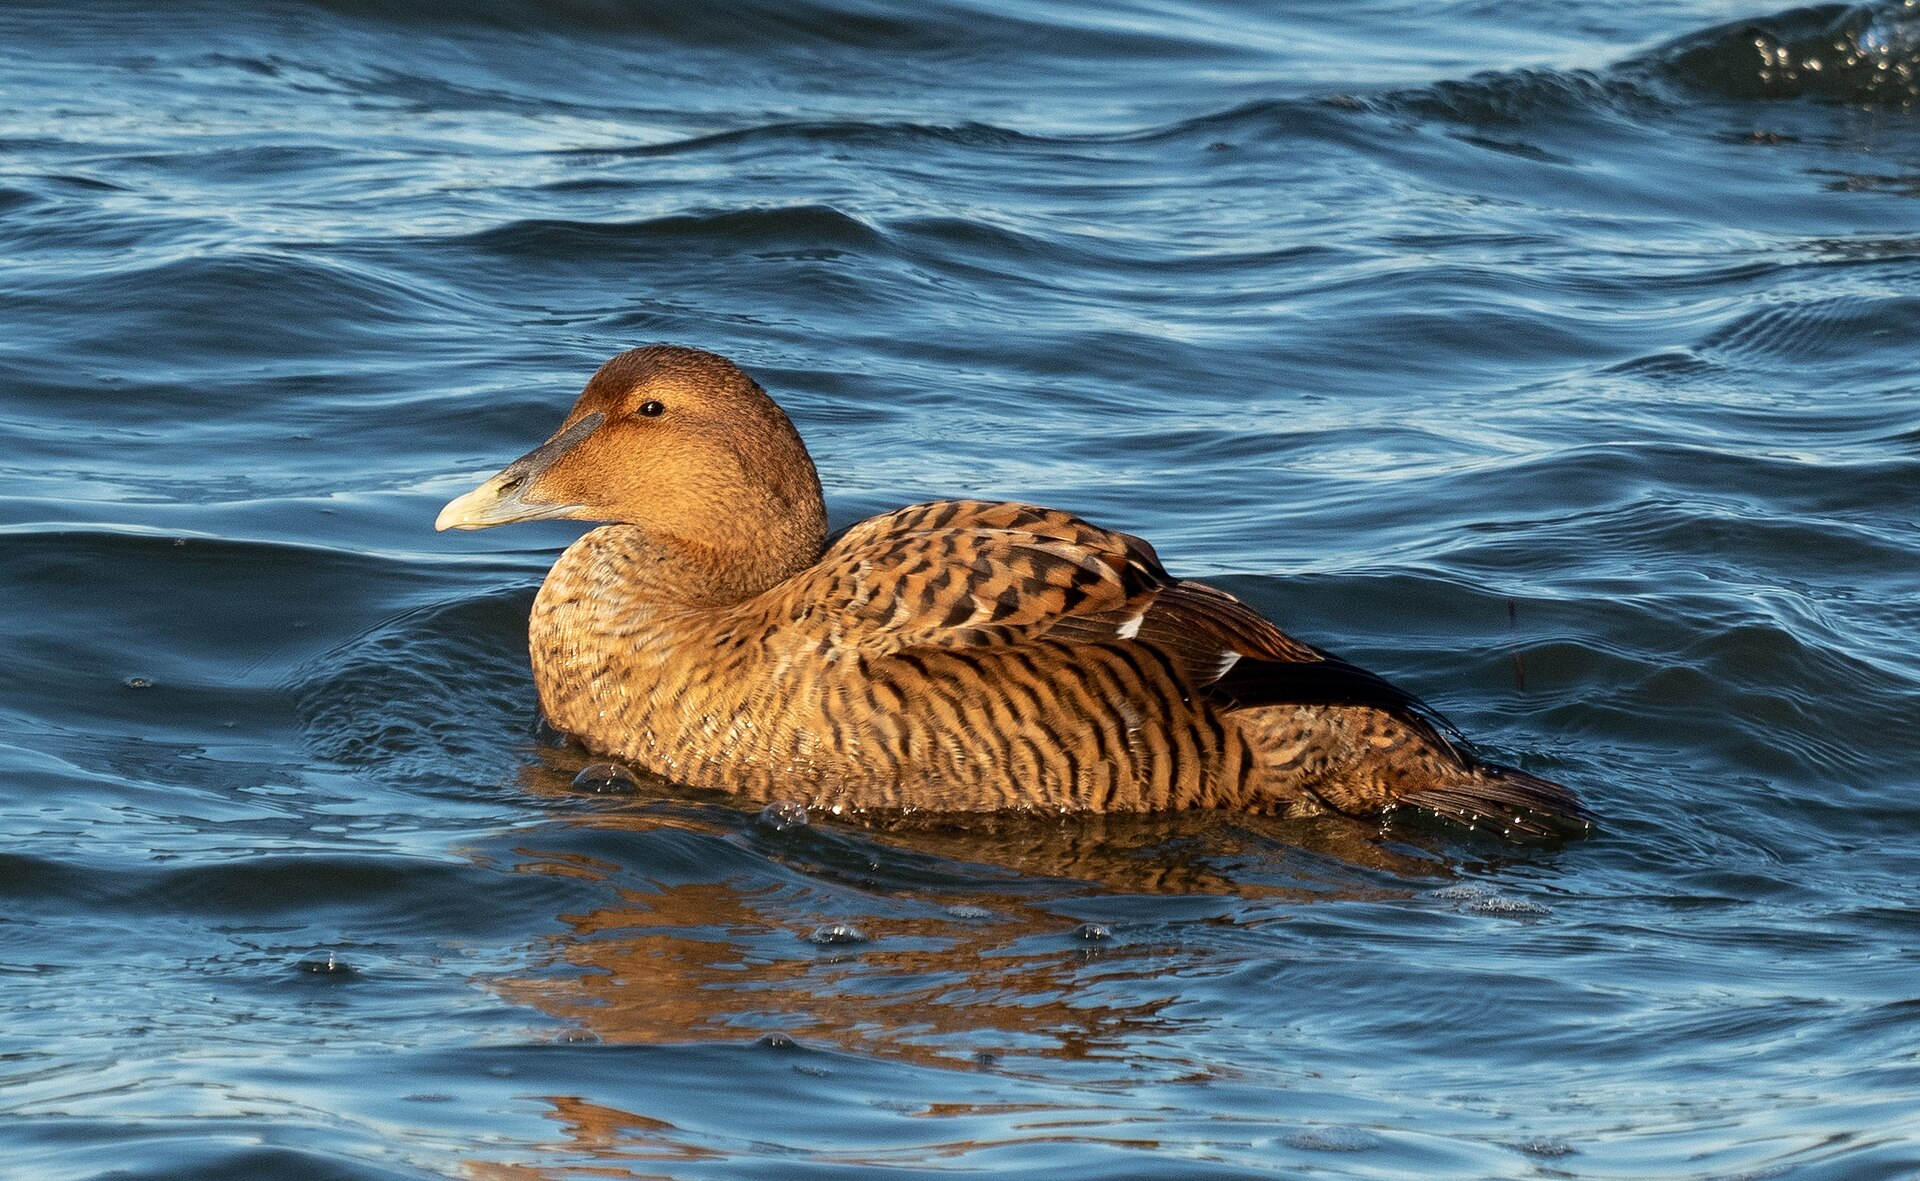
\includegraphics[width=0.7\linewidth, height=3cm, keepaspectratio]{Billeder/Dyr/Fugle/Aender/Dykaender/ederfugl_hun.jpg}
      \end{minipage}
    }%
    \vspace{0.05em}
    \footnotesize Han (kok) øverst, hun (høne) nederst
  \end{columns}
\end{frame}